\documentclass[11pt,a4paper]{article}
\usepackage{a4wide}
\usepackage{color}
\usepackage{graphicx}
% Default margins are too wide all the way around. I reset them here
%\setlength{\topmargin}{-.5in}
%\setlength{\textheight}{9in}
%\setlength{\oddsidemargin}{.125in}
%\setlength{\textwidth}{175mm}
\setlength{\parindent}{0cm}
\begin{document}
\title{COSC3500\\Serial Implementation Report}
\author{Anthony Vaccaro\\University of Queensland}

%\today
\maketitle
\begin{abstract}
This report introduces the concept of modelling forest fires with cellular
automata, and discusses an implementation of said model.
\end{abstract}


\newpage
\section{The Forest-Fire Model}

The Forest-Fire model is a cellular automaton-based model of a wild fire
spreading through a forest of trees or other plants. The model has a few
variants but typically follows these rules:

\begin{itemize}
\item An empty cell becomes a tree with probability p.
\item A tree becomes a burning tree with probability f.
\item A tree becomes a burning tree if its neighbours are burning.
\item A burning tree becomes an empty cell.
\end{itemize}
Where variables p and f can be adjusted to produce different patterns.

These simple rules can produce complex patterns and have lead to some research
into the area of modelling forest fires.

\newpage
\section{Algorithm used to represent model}

The algorithm chosen for this report and corresponding program is based on the
rules given above, with a few minor adjustments:

\begin{itemize}
\item Burning trees take l timesteps to become empty.
\item Trees with burning neighbours have probability c to catch fire.
\end{itemize}

This gives provides the simulation with four main variables to adjust - p, f,
l, and c.

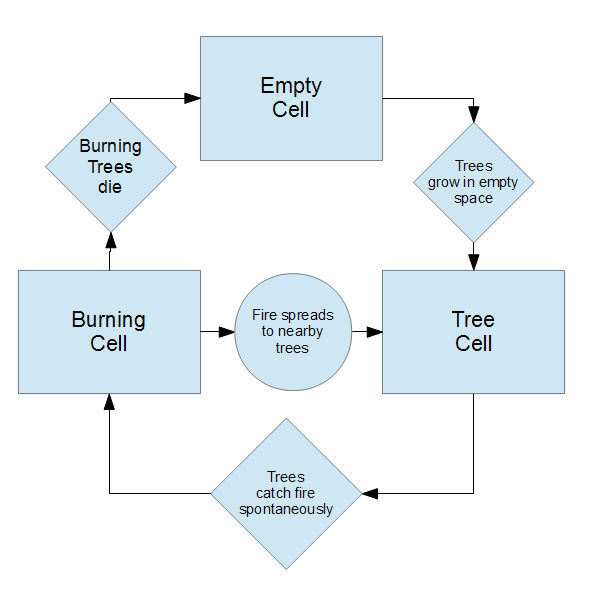
\includegraphics{tex/flowchart}

\newpage
\section{Implementation details}

The implementation was chosen to be written in C, based on the student's past
experience with programming. The implementation did not require any complex
programming techniques, although a few key points are worth discussing.

As much of this simulation relies on probabilities, the use of a random number
generator requires some thought. the \texttt{random()} function of the C
standard library was selected due to its ease of use and availability, but as
it is only a pseudo-random number generator, perhaps this could be changed in
later efforts. There are websites that provide "true randomness" based on
atmospheric noise\cite{random}, and perhaps data from this service could be
used and compared against the output of \texttt{random()}.

Exporting the output of the program was done via the use of
libpng\cite{libpng}, which can easily convert 2d arrays into pictures. Sample
code was used from a third party website in order to assist with this
process\cite{png}. After each timestep was completed, the grid of cells was
exported to an image, with pixels being coloured based on their status.

\newpage
\section{Verification of program's output correctness}

The implementation currently uses \texttt{random()} for its random number
generation, and this can be made deterministic by using a predefined seed with
the \textt{srandom()} function. This will be used to compare the results of
later optimisations and multiprocessing techniques.

\newpage
\section{Algorithm's performance while scaling with forest size}

As the algorithm operates on neighbours, which remain constant with an
increasing grid size, performance should scale linearly with number of cells in
the grid.

\begin{verbatim}

$ time ./forest 100 0 100
real    0m1.179s
user    0m0.433s
sys     0m0.046s

$ time ./forest 200 0 100
real    0m2.524s
user    0m1.802s
sys     0m0.113s

$ time ./forest 300 0 100

real    0m5.395s
user    0m4.500s
sys     0m0.172s



\end{verbatim}

\newpage
\section{Further Considerations}

\newpage

\begin{thebibliography}{99}

\bibitem{png}
"Write a PNG file using C and libpng", 2010 Ben Bullock
http://www.lemoda.net/c/write-png/

\bibitem{libpng}
"libpng Home Page", 2013 Greg Roelofs
http://www.libpng.org/pub/png/libpng.html

\bibitem{random}
"RANDOM.ORG - True Random Number Service", 2012 RANDOM.ORG
http://www.random.org/

\end{thebibliography}
\end{document}
    
    
